\subsection{Pathwise KL Regularization}\label{sec:pathwise_kl}

In behavior-regularized RL, previous methods typically regularize action distribution, i.e., the marginalized distribution $p^{\pi, s}_{0}$. Instead, we shift our attention to the KL divergence with respect to the diffusion path $a^{0:N}$, which can be further decomposed thanks to the Markov property: 
\begin{equation}\label{eq:pathwise_kl}
    \begin{aligned}
        &\KL{p^{\pi, s}_{0:N}}{p^{\nu, s}_{0:N}}\\
        &=\mathbb{E}\left[\log\frac{p^{\pi, s}_{0:N}(a^{0:N})}{p^{\nu, s}_{0:N}(a^{0:N})}\right]\\
        &=\mathbb{E}\left[\log \frac{p_N^{\pi,s}(a^N)\prod_{n=1}^Np_{n-1|n}^{\pi,s}(a^{n-1}|a^n)}{p_N^{\nu,s}(a^N)\prod_{n=1}^Np_{n-1|n}^{\nu,s}(a^{n-1}|a^n)}\right]\\
        &=\mathbb{E}\left[\log \frac{p^{\pi, s}_{N}(a^{N})}{p^{\nu, s}_{N}(a^{N})}+\sum_{n=1}^{N}\log\frac{p^{\pi, s,a^n}_{n-1|n}(a^{n-1})}{p^{\nu, s,a^n}_{n-1|n}(a^{n-1})}\right]\\
        &=\mathbb{E}\left[\sum_{n=1}^{N}\KL{p^{\pi, s,a^n}_{n-1|n}}{p^{\nu, s,a^n}_{n-1|n}}\right]. 
    \end{aligned}
\end{equation}
Here, the expectation is taken w.r.t. $a^{0:N}\sim p^{\pi, s}_{0:N}$, $p^{\nu}$ is the behavior diffusion policy trained via \eqref{eq:elbo} on the offline dataset $\mathcal{D}$ to approximate the data-collection policy, and the last equation holds due to $p_N^{\pi,s}=p_{N}^{\nu,s}=\mathcal{N}(0, I)$. In the following, we abbreviate $\KL{p^{\pi, s,a^n}_{n-1|n}}{p^{\nu, s,a^n}_{n-1|n}}$ with $\ell^{\pi,s}_{n}(a^n)$.

Based on this decomposition, we present the pathwise KL-regularized RL problem.
\begin{definition}\label{problem:pathwise_kl_brl}
    \textit{(Pathwise KL-Regularized RL)} Let $p^{\nu}$ be the behavior diffusion process. The pathwise KL-regularized RL problem seeks to maximize the following objective
    \begin{equation}
    \label{eq:pathwise_kl_obj}
        \max_{p^\pi}\  \mathbb{E}\left[\sum_{t=0}^\infty \gamma^t\left(R(s_t,a_t^0)-\eta\sum_{n=1}^N\ell_{n}^{\pi,s_t}(a_t^n)\right)\right].
    \end{equation}
where the expectation is taken w.r.t. trajectories following $p^\pi$ and the dynamics $T$.
\end{definition}

Although our problem calculates the accumulated discrepancies along the diffusion path as penalties, it actually preserves the same optimal solution to \eqref{eq:brl_obj}, which only regularizes the action distribution at diffusion step $n=0$. The following theorem captures the equivalence. 
\begin{theorem}{(Proof in Appendix~\ref{thm:pathwise_kl_equivalence})}
    Let $p^\nu$ be the behavior diffusion process. The optimal diffusion policy $p^{*}$ of the pathwise KL-regularized RL problem in \eqref{eq:pathwise_kl_obj} is also the optimal policy $\pi^*$ of the KL regularized objective in \eqref{eq:brl_obj}, in the sense that $\pi^*(a|s)=\int p^{*, s}_{0:N}(a^{0:N})\delta(a-a^0)\mathrm{d}a^{0:N} \ \forall s\in\mathcal{S}$, where $\delta$ is the Dirac delta function. 
\end{theorem}
% \begin{proof}
%     Proof can be found in Appendix~\ref{thm:pathwise_kl_equivalence}. 
% \end{proof}

That said, we can safely optimize \eqref{eq:pathwise_kl_obj} and ultimately arrive at the solution that also maximizes the original KL-regularized RL problem. As will be demonstrated in the following sections, our formulation of the penalty leads to an analytical and efficient algorithm, since each single-step reverse transition is tractable.

\begin{figure*}
    \centering
    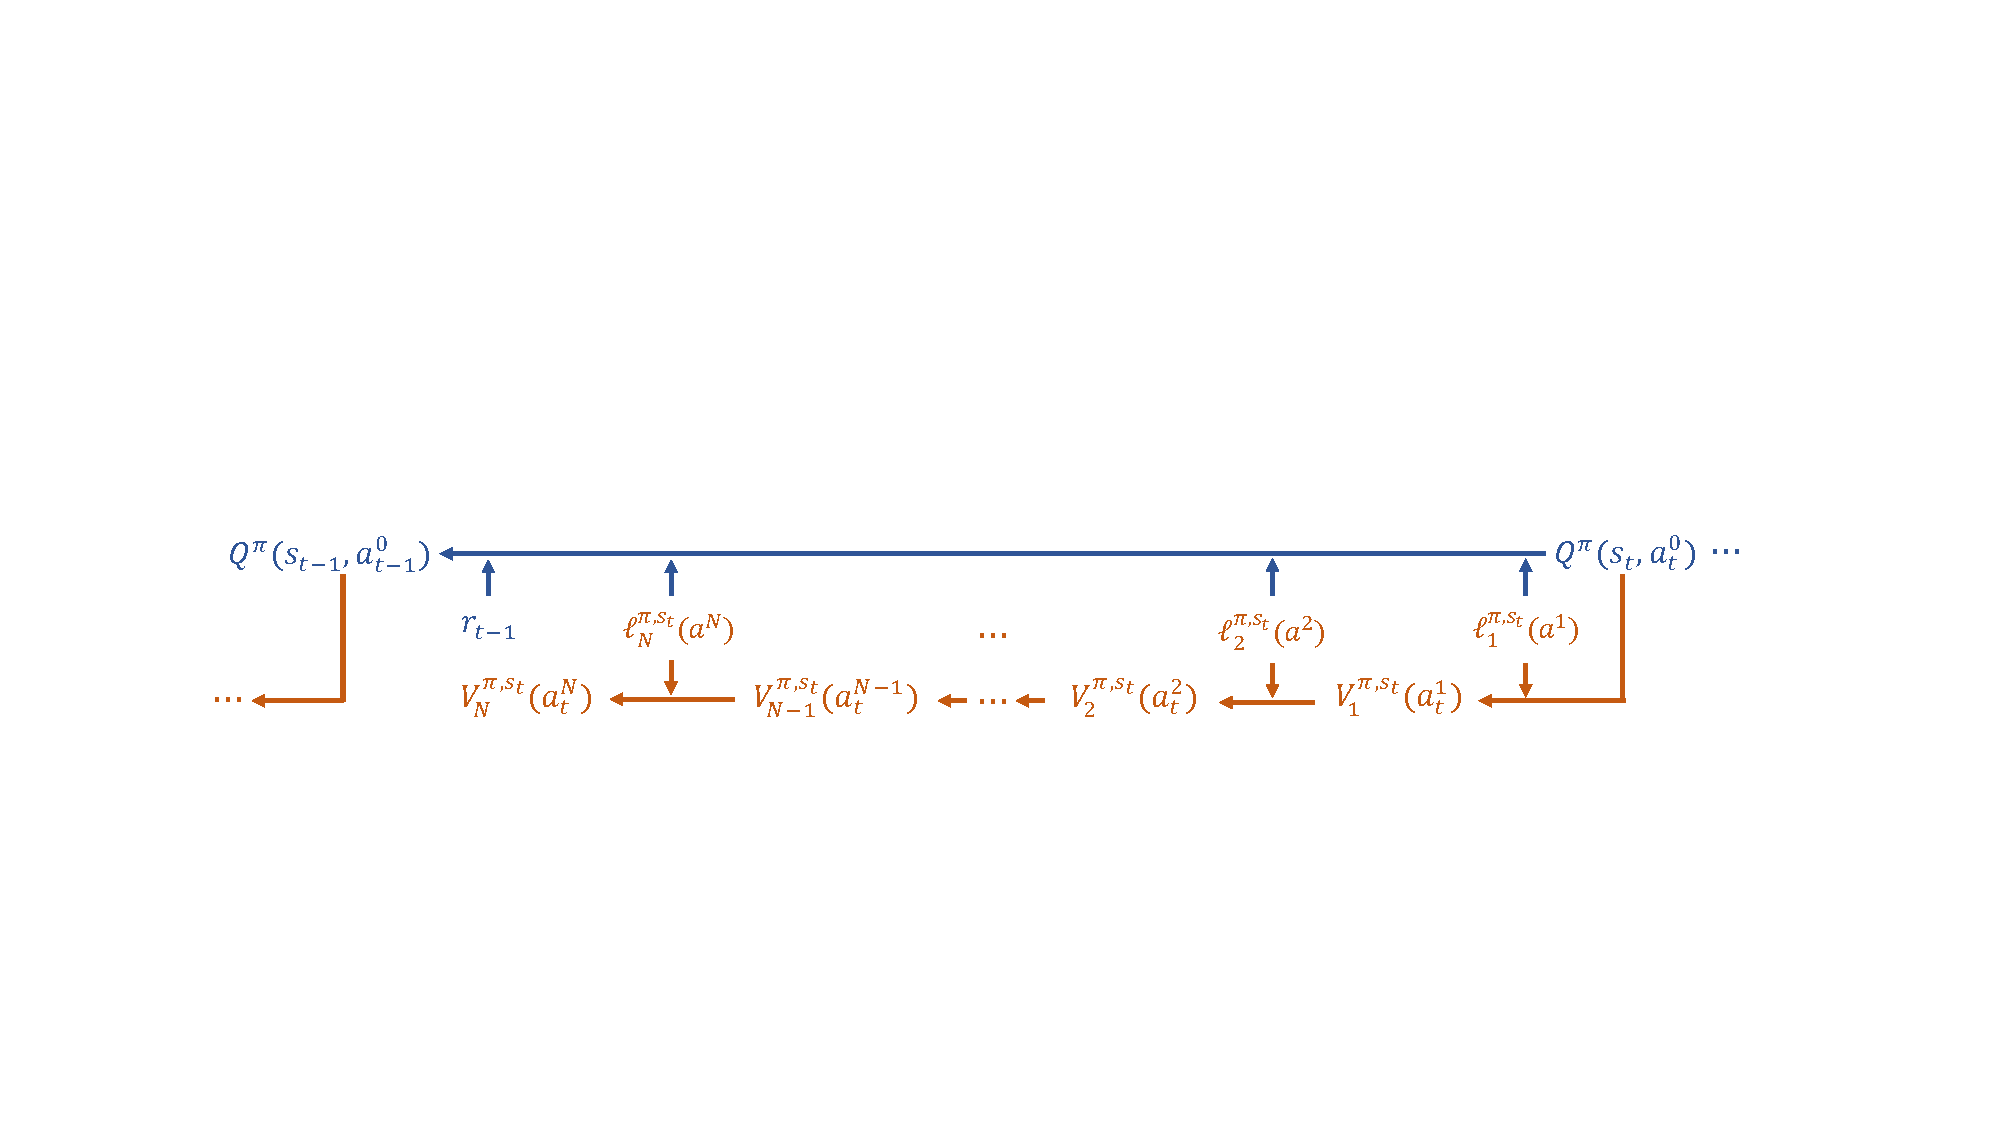
\includegraphics[width=0.9\linewidth]{images/intro_backup.pdf}
    \caption{Semantic illustration of the TD backup for the Q-value function $Q^\pi$ (blue) and diffusion value function $V^{\pi,s}_n$ (orange). The update of $Q^\pi$ (\eqref{eq:upper_critic}) requires reward, penalties along the diffusion trajectory, and the Q-values at the next state. The update of $V^{\pi,s}_n$ (\eqref{eq:intermediate_value}) involves the single-step penalty and the diffusion value at the next diffusion step $n-1$. }
    \label{fig:intro_backup}
\end{figure*}

\subsection{Actor-Critic across Two Time Scales}
To solve the pathwise KL-regularized RL (\eqref{eq:pathwise_kl_obj}), we can employ an actor-critic framework. Specifically, we maintain a diffusion policy $p^\pi$ and a critic $Q^\pi$. The update target of the critic $Q^\pi$ is specified as the standard TD target in the environment MDP:
\begin{equation}\label{eq:upper_critic}
\begin{aligned}
    \scalemath{0.95}{\mathcal{B}^\pi Q^\pi(s,a)=R(s, a)+\gamma \mathbb{E}\Big[Q^\pi(s', a'^0)-\eta\sum_{n=1}^N\ell^{\pi,s'}_{n}(a'^n)\Big],}
\end{aligned}
\end{equation}

i.e., we sample diffusion paths $a'^{0:N}$ at the next state $s'$, calculate the Q-values $Q^\pi(s', a'^0)$ and the accumulated penalties along the path, and perform a one-step TD backup. For the diffusion policy, its objective can be expressed as:
\begin{equation}\label{problem:path_diff}
    \begin{aligned}
        \max_{p^{\pi,s}}\ 
        \underset{{a^{0:N}\sim p^{\pi,s}_{0:N}}}{\mathbb{E}}\left[Q^\pi(s, a^0)-\eta\sum_{n=1}^N\ell^{\pi,s}_{n}(a^n)\right].
    \end{aligned}
\end{equation}

At first glance, one might treat the pathwise KL as a whole and optimize the diffusion policy by back-propagating the gradient throughout the sampled path $a^{0:N}$, similar to Diffusion-QL~\citep{dql}. Nevertheless, this requires preserving the computation graph of all diffusion steps and therefore incurs considerable computational overhead. Moreover, the inherent stochasticity of the diffusion path introduces significant variance during optimization, which can hinder the overall performance. 

Instead, we opt for a bi-level TD learning framework. The upper level updates $Q^\pi$ according to \eqref{eq:upper_critic} and operates in the environment MDP. In the lower level, we maintain \textit{diffusion value functions} $V^{\pi, s}_n(a^n)$, which are designed to estimate the values at intermediate diffusion steps. The TD target of $V^{\pi,s}_{n}$ is specified as:
\begin{equation}\label{eq:intermediate_value}
    \begin{aligned}
        &\mathcal{T}_0^{\pi}V_0^{\pi,s}(a^0)=Q^\pi(s,a^0),\\
        &\mathcal{T}_n^{\pi}V_n^{\pi,s}(a^n)=-\eta \ell^{\pi,s}_n(a^n)+\underset{ p^{\pi,s,a^n}_{n-1|n}}{\mathbb{E}}\left[V_{n-1}^{\pi,s}(a^{n-1})\right].
    \end{aligned}
\end{equation}
Intuitively, $V^{\pi, s}_n(a^n)$ receives the state $s$, intermediate generation result $a^n$, and the diffusion step $n$ as input, and estimates the expected cumulative penalties of continuing the diffusion path at $a^n$ and step $n$. It operates completely inside each environment timestep and performs TD updates across the diffusion steps. The semantic illustration of the value function backups is presented in Figure~\ref{fig:intro_backup}. The following proposition demonstrates the convergence of policy evaluation. 

With the help of $V^{\pi, s}_n$, we can update the policy according to
\begin{equation}\label{problem:step_diff}
    \begin{aligned}
    &\max_{p^{\pi,s,a^n}_{n-1|n}}\ \ -\eta\ell^{\pi,s}_n(a^n) + \underset{p^{\pi,s,a^n}_{n-1|n}}{\mathbb{E}}\left[V^{\pi,s}_{n-1}(a^{n-1})\right].
    \end{aligned}
\end{equation}

\begin{algorithm}[t]
\caption{Behavior-Regularized Diffuion Policy Optimization (\texttt{BDPO})}
\label{code}
\textbf{Input}: Offline dataset $\mathcal{D}$, initialized diffusion policy $p^\pi$ and $p^\nu$, Q-value networks $Q_{\psi_k}$, diffusion value networks $V_{\phi_k}$.

\begin{algorithmic}[1]
\STATE {\color{gray}// Pretrain $p^\nu$}
\STATE Pretrain the behavior diffusion policy $p^\nu$ via \eqref{eq:elbo}
\STATE Initialize $p^\pi$ with $p^\nu$
\STATE {\color{gray}// Train $p^\pi$}
\FOR{$i=1, 2, \cdots, N_{\text{total\_steps}}$}
\STATE Sample minibatch $B=\{(s_i, a_i, s'_i, r_i)\}_{i=1}^{|B|}$ from $\mathcal{D}$
\STATE Update $\{Q_{\psi_k}\}_{k=1}^K$ via \eqref{eq:critic_loss} using $B$
\STATE Extend each $(s_i,a_i,s'_i,r_i)$ in $B$ by sampling $n\sim U[1, N]$ and $a^{n}_t\sim q_{n|0}(\cdot|a_t)$
\STATE Update $\{V_{\phi_k}\}_{k=1}^K$ via \eqref{eq:critic_loss} using $B$
\IF{$i$ \% actor\_update\_interval == 0}
\STATE Update $p^\pi$ by performing gradient ascend with the objective defined in \eqref{problem:step_diff} and $B$
\ENDIF
\ENDFOR
\end{algorithmic}
\end{algorithm}

Note that the maximization is over every state $s$, diffusion step $n$, and intermediate action $a^n$. In this way, we only require single-step reverse diffusion during policy improvement, providing an efficient solution to the problem defined in~\eqref{problem:step_diff}.

Through simple recursion, we can demonstrate that updating $p^{\pi}$ with \eqref{problem:step_diff} leads to the same optimal solution to the original policy objective \eqref{problem:path_diff}.

\begin{assumption}
\label{ass}
Let $\Pi$ be the set of admissible diffusion policies satisfying $\forall\,p^\pi\in\Pi,\;\forall\,s\in\mathcal{S}$,
\[
\sup_{a^0\in\mathcal{A}}\;\frac{\pi(a^0|s)}{\nu(a^0|s)}=\frac{\int p_{0:N}^{\pi,s}(a^{0:N})\mathrm{d}a^{1:N}}{\int p_{0:N}^{\nu,s}(a^{0:N})\mathrm{d}a^{1:N}}<\infty,
\]
where $p^\nu$ is the behavior diffusion policy.
\end{assumption}
\begin{proposition}{(Soft Policy Improvement, proof in Appendix~\ref{proposition:policy_improvement})}\label{main_proposition:policy_improvement}
Let $p^{\pi_{\textrm{new}}}$ be the optimizer of the problem defined in \eqref{problem:step_diff}. Under Assumption~\ref{ass}, $V^{\pi_{\textrm{new}},s}_n(a^n)\geq V^{\pi_{\textrm{old}},s}_n(a^n)$ holds for all $n\in\{0, 1, \ldots, N\}$ and $(s, a)\in\mathcal{S}\times\mathcal{A}$.
\end{proposition}
% \begin{proof}
%     Proof can be found in Appendix~\ref{proposition:policy_improvement}. 
% \end{proof}

Combining Proposition~\ref{main_proposition:policy_improvement} and a similar convergence argument in Soft Actor Critic~\cite{sac}, we obtain that the policy is guaranteed to improve w.r.t. the pathwise KL problem in Definition~\ref{problem:pathwise_kl_brl}. 

\begin{proposition}{(Policy Iteration, proof in Appendix~\ref{proposition:policy_iteration})}
Under Assumption~\ref{ass}, repeated application of soft policy evaluation in \eqref{eq:upper_critic} and \eqref{eq:intermediate_value} and soft policy improvement in \eqref{problem:step_diff} from any $p^\pi\in\Pi$ converges to a policy $p^{\pi^*}$ such that $V_n^{\pi^*,s}(a)\geq V_n^{\pi,s}(a)$ for all $p^\pi\in\Pi$, $n\in\{0,1,\ldots,N\}$, and $(s,a)\in\mathcal{S}\times\mathcal{A}$.
\end{proposition}
% \begin{proof}
% Proof can be found in Appendix~\ref{proposition:policy_iteration}. 
% \end{proof}

\begin{figure*}
    \centering
    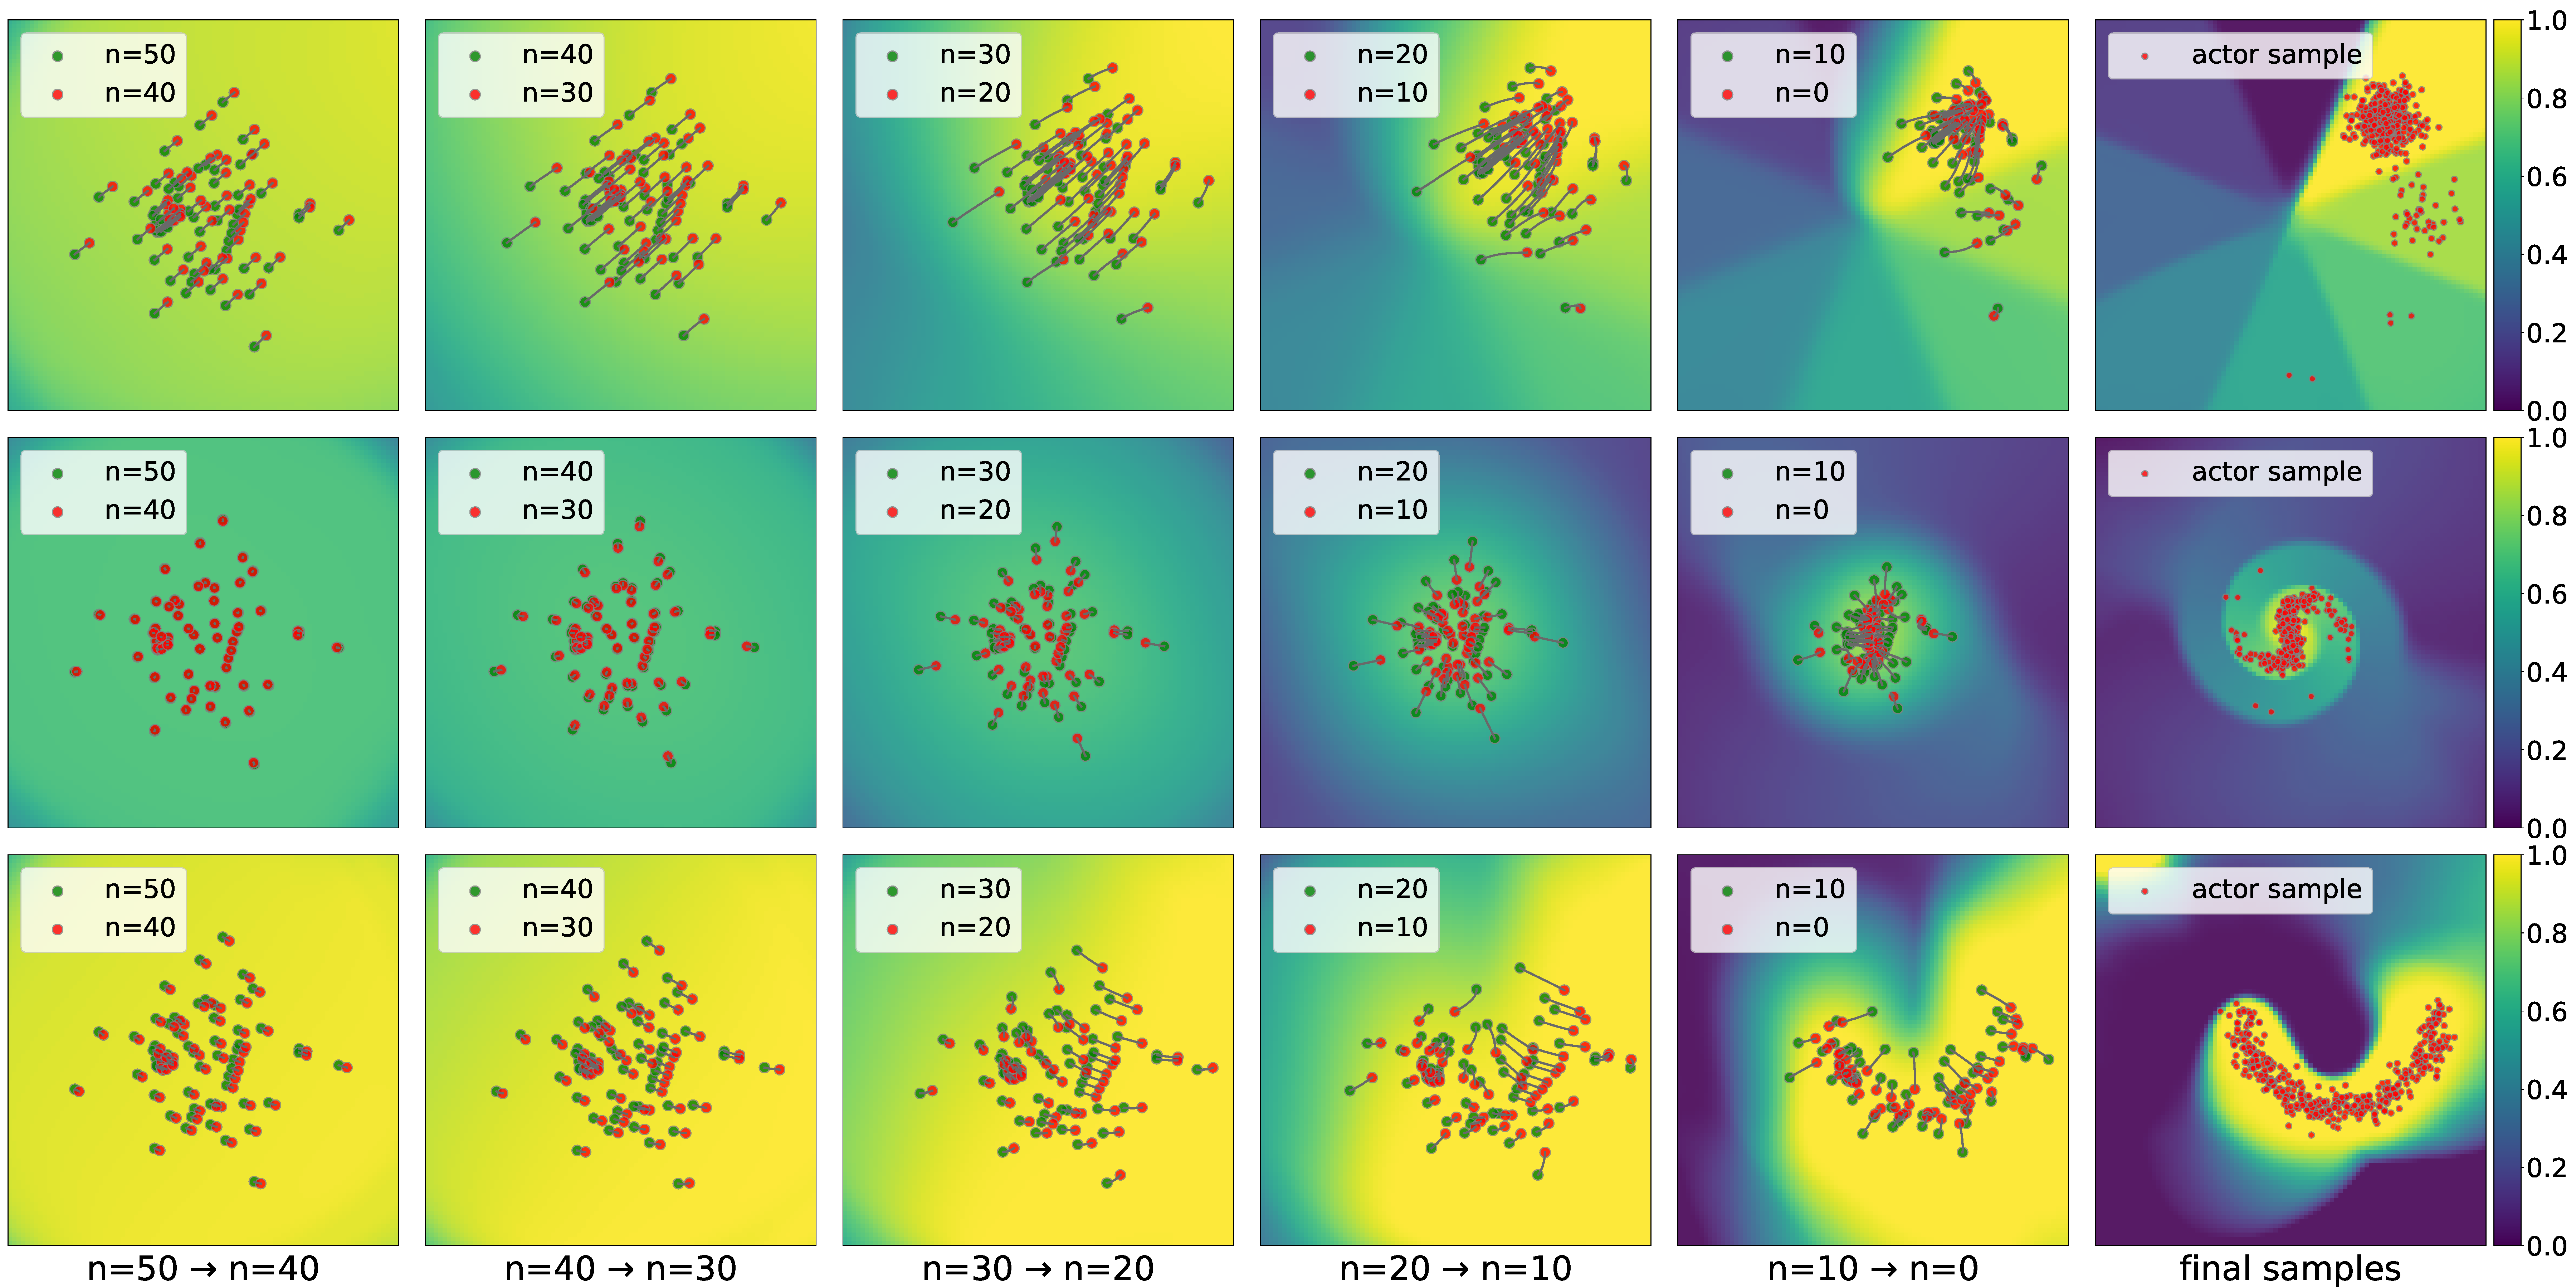
\includegraphics[width=0.95\linewidth]{images/5.1_actor.pdf}
    \caption{Generation paths of \algbb on the \textit{8gaussian} (top), \textit{2spirals} (middle), and \textit{moons} (down) datasets. The regularization strength is set to $\eta=0.06$, which is identical to Figure~\ref{fig:2d_data}. The first five columns depict the diffusion generation process at different time intervals, with green dots indicating the starting points of these intervals, red dots indicating the ending points, and grey lines in between representing intermediate samples. The background color depicts the output from the diffusion value functions $V^{\pi,s}_n$ in the entire 2D space. The rightmost figures depict the final action samples. We use DDIM sampling~\citep{ddim} for better illustration.}\label{fig:2d_actor}
\end{figure*}

\begin{figure}[h]
    \centering
    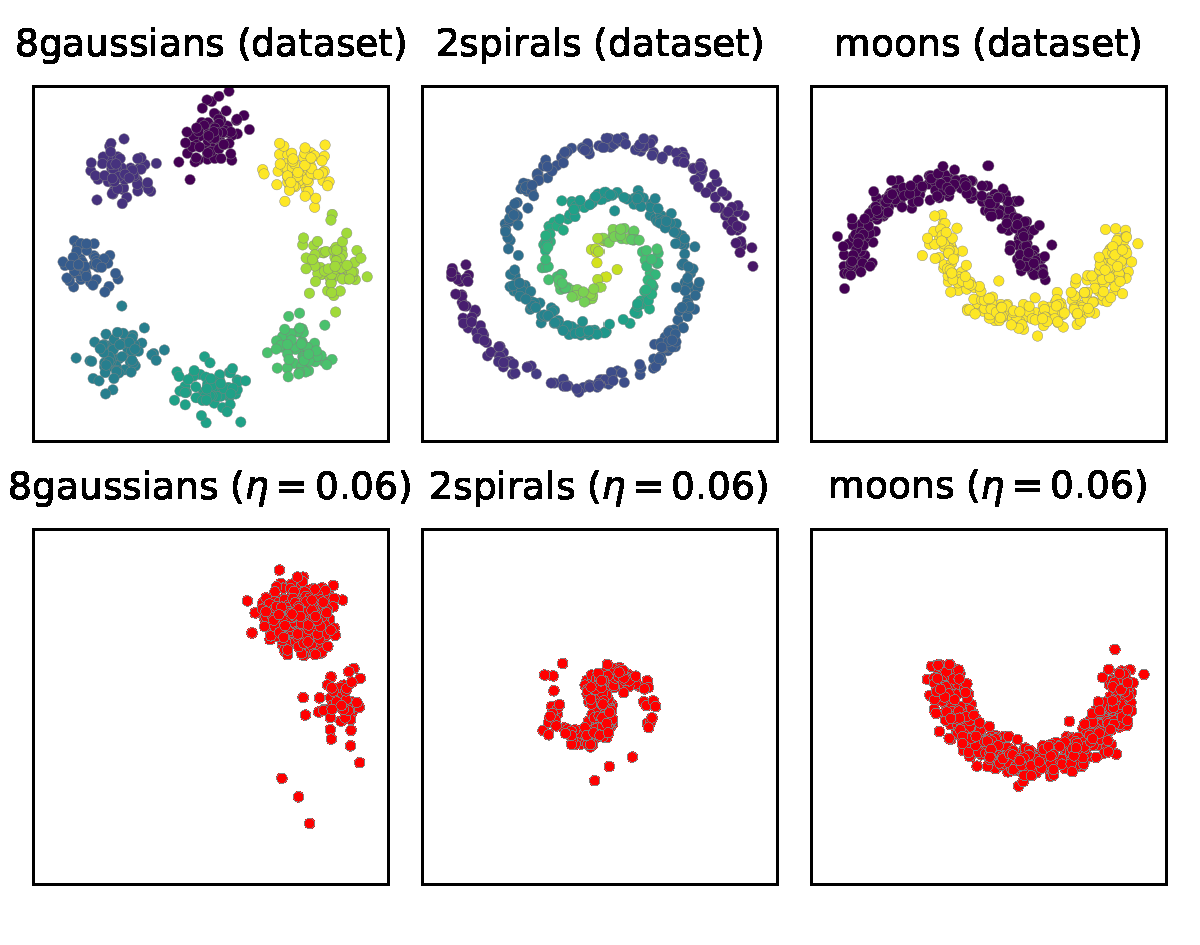
\includegraphics[width=0.9\linewidth]{images/5.1_data.pdf}
    \caption{Illustration of the \textit{8gaussians}, \textit{2spirals}, and \textit{moons} datasets. The top row depicts the original data distribution $p_{\text{data}}$, while the second row depicts the target distribution $p_{\text{target}}$ at $\eta=0.06$ by re-sampling data points according to their energies.}\label{fig:2d_data}
\end{figure}


\textbf{Remark (Actor-critic across two time scales). }Our treatment of the environment MDP and the (reverse) diffusion MDP resembles DPPO~\citep{dppo}, which unfolds the diffusion steps into the environment MDP and employs the PPO~\citep{ppo} algorithm to optimize the diffusion policy in the extended MDP. Compared to DPPO, our method adds a penalty in each diffusion step to implement behavior regularization. Besides, we maintain two types of value functions to account for both inter-timestep and inner-timestep policy evaluation, thereby offering low-variance policy gradients. 

\subsection{Practical Implementation}
\textbf{Calculation of KL Divergence. }
Since each single-step reverse transition $p_{n-1|n}^{\pi,s,a_n}$ is approximately parameterized as an isotropic Gaussian distribution (\eqref{eq:reverse_diff}), the KL divergence is analytically expressed as
\begin{equation}
    \begin{aligned}
        \KL{p^{\pi, s,a^n}_{n-1|n}}{p^{\nu, s,a^n}_{n-1|n}}=\frac{\|\mu^{\pi,s}_n(a^n)-\mu^{\nu,s}_n(a^n)\|^2}{2\sigma_n^2}.
    \end{aligned}
\end{equation}
That is, each penalty term is simply the discrepancy between the mean vectors of the reverse transitions, weighted by a factor depending on the noise schedule. The transition of the reverse process becomes Gaussian exactly in the continuous limit, in which case, the KL divergence can be computed through Girsanov's theorem~\citep{oksendal2013stochastic}, and the sum of mean squared errors (MSEs) is replaced by an integral \cite{minde}. In Appendix~\ref{appsec:continuous_time}, we demonstrate that the pathwise KL is consistent with the result from Girsanov's theorem in the limit of infinitesimal diffusion step size. 


\begin{table*}[h!]
\centering
\setlength{\tabcolsep}{1.1mm}{}
\caption{Comparison of \algbb and various baseline methods on locomotion-v2 and antmaze-v0 datasets from D4RL. We use `m' as the abbreviation for medium, `r' for replay, and `e' for expert. The performances of the baseline methods are taken from their original paper. For \algbb, we report the average and the standard deviation of the performances across 10 evaluation episodes (100 for antmaze datasets) and 5 seeds. We bold values that are within $95\%$ of the top-performing method.}
\label{tab:d4rl}
\small{
\begin{tabular}{lccccccccccc|r}
\toprule
\textbf{Dataset} & \textbf{CQL} & \textbf{IQL} & \textbf{DD} & \textbf{SfBC} & \textbf{IDQL-A} & \textbf{QGPO} & \textbf{SRPO} & \textbf{DTQL} & \textbf{Diffusion-QL} & \textbf{EDP} & \textbf{DAC} & \textbf{BDPO (Ours)}\\ 
\midrule
halfcheetah-m & 44.0 & 47.4 & 49.1 & 45.9 & 51.0 &  54.1 & 60.4 & 57.9 & 51.1 
& 52.1 & 59.1 & \textbf{71.2$\pm$0.9}\\ 
hopper-m & 58.5 & 66.3 & 79.3 & 57.1 & 65.4 & \textbf{98.0} & 95.5 & \textbf{99.6} & 90.5 & 81.9 & \textbf{101.2} & \textbf{100.6$\pm$0.7}\\ 
walker2d-m & 72.5 & 78.3 & 82.5 & 77.9 & 82.5 & 86.0 & 84.4 & 89.4 & 87.0 & 86.9 & \textbf{96.8} & \textbf{93.4$\pm$0.5}\\ 
halfcheetah-m-r & 45.5 & 44.2 & 39.3 & 37.1 & 45.9 & 47.6 & 51.4 & 50.9 & 47.8 & 49.4 &55.0 & \textbf{58.9$\pm$0.9}\\ 
hopper-m-r & 95.0 & 94.7 & \textbf{100.0} & 86.2 & 92.1 & 96.9 & \textbf{101.2} & \textbf{100.0} & 
\textbf{101.3} & \textbf{101.0} & \textbf{103.1} & \textbf{101.4$\pm$0.5}\\ 
walker2d-m-r & 77.2 & 73.9 & 75.0 & 65.1 & 85.1 & 84.4 & 84.6 & 88.5 & \textbf{95.5} & \textbf{94.9} & \textbf{96.8} & \textbf{95.5$\pm$1.6}\\ 
halfcheetah-m-e & 91.6 & 86.7 & 90.6 & 92.6 & 95.9 & 93.5 & 92.2 & 92.7 & 96.8& 95.5 &99.1  & \textbf{108.7$\pm$0.9}\\ 
hopper-m-e & \textbf{105.4} & 91.5 & \textbf{111.8} & \textbf{108.6} & \textbf{108.6} & \textbf{108.0} & 
100.1 &\textbf{109.3} & \textbf{111.1} & 
97.4 & \textbf{111.7} & \textbf{111.3$\pm$0.2}\\ 
walker2d-m-e & 108.8 & \textbf{109.6} & 108.8 & \textbf{109.8} & \textbf{112.7} & \textbf{110.7} & \textbf{114.0} & \textbf{110.0} & \textbf{110.1} & \textbf{110.2} & \textbf{113.6} & \textbf{115.6$\pm$0.4}\\ 
\midrule
\textbf{locomotion sum} & 698.5 & 749.7 & 736.2 & 680.3 & 739.2 & 779.2 & 783.8 & 798.3 & 791.2 & 769.3 & 836.4 & \textbf{856.7}\\ 
\midrule
\midrule
antmaze-u & 74.0 & 87.5 & - & 92.0 & 94.0 & \textbf{96.4} & 90.8 & \textbf{94.8} & 93.4 & 94.2 & \textbf{99.5} & \textbf{98.4$\pm$1.5} \\ 
antmaze-u-div & \textbf{84.0} & 62.2 & - & \textbf{85.3} & 80.2 & 74.4 & 59.0 & 78.8 & 66.2 & 79.0 & \textbf{85.0} & \textbf{83.0$\pm$12.4}\\ 
antmaze-m-play & 61.2 & 71.2 & - & 81.3 & 84.5 & 83.6 & 73.0 & 79.6 & 
76.6 & 81.8 & 85.8 & \textbf{92.0$\pm$2.9}\\ 
antmaze-m-div & 53.7 & 70.0 & - & 82.0 & 84.8 & 83.8 & 65.2 & 82.2 & 78.6 & 
82.3 & 84.0 & \textbf{93.2$\pm$2.8}\\ 
antmaze-l-play & 15.8 & 39.6 & - & 59.3 & 63.5 & \textbf{66.6} & 38.8 & 52.0 & 46.4 & 42.3 & 50.3 & \textbf{69.0$\pm$8.0}\\ 
antmaze-l-div & 14.9 & 47.5 & - & 45.5 & 67.9 & 64.8 & 33.8 & 54.0 & 56.6 & 60.6 & 55.3 & \textbf{84.0$\pm$3.2}\\ 
\midrule
\textbf{antmaze sum} & 303.6 & 378.0 & - & 445.4 & 474.9  & 469.6 & 360.6 & 441.4 & 417.8 & 440.2 & 459.9 & \textbf{519.6}\\ 
\bottomrule
\end{tabular}
}
\end{table*}


\textbf{Selection of States, Diffusion Steps and Actions. }The policy improvement step requires training $V^{\pi,s}_n$ and improving $p^\pi$ on every $(s, a^n, n)$ triplet sampled from the on-policy distribution of $p^\pi$. However, we employ an off-policy approach, by sampling $(s, a)$ from the dataset, $n$ according to the Uniform distribution $U[1, N]$ and $a^n$ according to $q_{n|0}(\cdot|a)$, which we found works sufficiently well in our experiments. We note that on-policy sampling $(s, a^n, n)$ may further benefit the performance at the cost of sampling and restoring these triplets on the fly, similar to what iDEM~\citep{idem} did in its experiments. 

\textbf{Lower-Confidence Bound (LCB) Value Target. }Following existing practices~\citep{dpqe,dac}, we use an ensemble of $K=10$ value networks $\{\psi_k, \phi_k\}_{i=k}^{K}$ for both $V^{\pi,s}_{n}$ and $Q^\pi$ and calculate their target as the LCB of \eqref{eq:upper_critic} and \eqref{eq:intermediate_value}:
\begin{equation}
\begin{aligned}
    y_Q&=\mathrm{Avg}_k[\mathcal{B}^\pi Q^\pi_{\bar{\psi}_k}]-\rho \sqrt{\mathrm{Var}_k[\mathcal{B}^\pi Q^\pi_{\bar{\psi}_k}]},\\
    y_V&=\mathrm{Avg}_k[\mathcal{T}_n^\pi V^{\pi,s}_{n,\bar{\phi}_k}]-\rho \sqrt{\mathrm{Var}_k[\mathcal{T}_n^\pi V^{\pi,s}_{n,\bar{\phi}_k}]},
\end{aligned}
\end{equation}
where $\bar{\phi}_k$ and $\bar{\psi}_k$ are exponentially moving average versions of the value networks, and $\mathrm{Avg},\mathrm{Var}$ denote averages and variances respectively. The objectives for value networks are to minimize the mean-squared error between the prediction and the target:
\begin{equation}\label{eq:critic_loss}
    \begin{aligned}
        \mathcal{L}(\{\psi_k\}_{k=1}^{K})&=\mathbb{E}_{(s, a, s',r)\sim\mathcal{D}}\left[\sum_{k=1}^K(y_Q - Q^\pi_{\psi_k}(s, a))^2\right],\\
        \mathcal{L}(\{\phi_k\}_{k=1}^{K})&=\mathbb{E}_{(s, a)\sim\mathcal{D}, n,a^n}\left[\sum_{k=1}^K(y_V - V^{\pi,s}_{n,\phi_k}(a^n))^2\right],
    \end{aligned}
\end{equation}
where $n$ is sampled from $U[1, N]$ and $a^n$ from $q_{n|0}(\cdot|a)$. 

The pseudo-code for \algbb is provided in Algorithm~\ref{code}.
